\section{Generierungsphase}

\begin{figure}[htbp] 
	\centering
	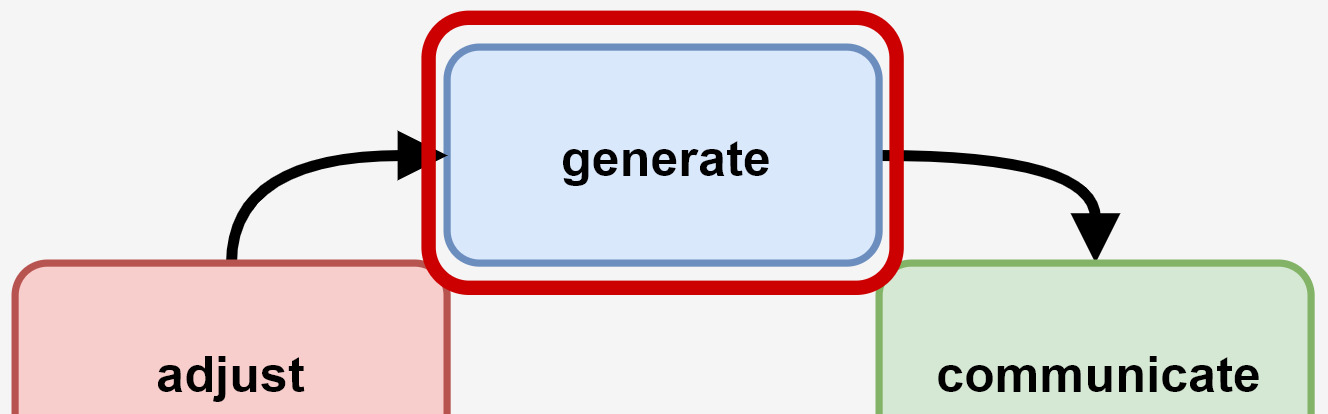
\includegraphics[width=0.75\textwidth]{contents/images/SmartGrazerSectionGenerate}
	\caption{SmartGrazer: Auszug Generierungsphase}
	\label{fig:SmartGrazerSectionGenerate}
\end{figure}

Dieses Kapitel erläutert die in Abbildung \ref{fig:SmartGrazerBirdView} blau gekennzeichnete ``generate''-Phase. Als Generatoren sind zwei Ansätze implementiert worden: Zum Einen wird ein kontextfreier Payload-Generator verwendet, auf dessen Generierungsprozess kein Einfluss genommen werden kann und zum Anderen wird ein kontextbezogener Generator implementiert, dessen Generierungsprozess von der Reaktion der Webseite abhängt.

Es wird im Folgenden der kontextfreie Generator ``Dharma'' vorgestellt, der im späteren Verlauf durch eine \gls{Adapter}-Klasse von SmartGrazer verwendet werden kann, um Payloads zu generieren. Hierzu wird für Dharma eine gesonderte Grammatikdefinition definiert, sodass die generierten Payloads von SmartGrazer interpretiert werden können.

\FloatBarrier

%%%%%%%%%% Dharma

\subsection{Dharma als kontextfreier Payload Generator}\label{Dharma}

Zunächst wird anhand eines Beispiels erklärt, wie Definitionsdateien für Grammatiken erstellt und von Dharma interpretiert werden. Anschließend wird die erstellte XSS-Grammatikdefinition für Dharma anhand von Beispielen näher betrachtet und erklärt.

\subsubsection{Definitionen von Grammatiken}

Wie bereits Kapitel \ref{ssec:grammar-based-approaches} erwähnt, gibt es bereits mehrere Implementierungen von kontextfreien Payload-Generatoren. Dharma ist ein Open Source Projekt von Mozilla und wurde für das Testen von WebAPIs entwickelt. Diese werden oft in Form einer \ac{IDL} definiert. Eine IDL stellt im Grunde eine Grammatik dar. Als Referenz zum kontextbezogenen Ansatz dieser Arbeit wurde für Dharma eine kontextfreie \ac{XSS}-Grammatik definiert und getestet. Um eine Wissensgrundlage zu schaffen, wird zunächst die Grundfunktion einer Definitionsdatei erklärt.

\newpage
\subsubsection{Ein Minimalbeispiel: minimal.dg}

Der Quelltextauszug \ref{lst:minimal.dg} stellt ein Minimalbeispiel einer Dharma-Grammatik dar. Die hier gezeigte Grammatik veranschaulicht eine Einstiegsregel, die anschließend zwei möglichen Pfaden folgen kann.

\begin{lstlisting}[caption={Dharma: Grundaufbau einer Grammatikdefinition},label=lst:minimal.dg]
%section% := value

rule :=
hello world
+hello+ hello world

hello :=
hello
+hello+ hello

%section% := variance
main :=
+rule+
\end{lstlisting}

In der letzten Zeile der oben dargestellten Definitionsdatei wird die auszuführende Regel der Grammatik bestimmt. Regeln werden durch die Zuweisung ``:=''\footnote{
Leerzeichen sind nur vor und nach dem Definitionssymbol ``:='' erlaubt. Ansonsten kann Dharma die Definitionsdatei nicht interpretieren.} bestimmt und mittels ``+Regelname+'' aufgerufen. In Beispiel \ref{lst:minimal.dg} ist die Einstiegsregel \textbf{rule}. Wird anschließend Zeile vier ausgewählt, gibt Dharma ``hello world'' aus (Pfad 1). Im anderen Fall wird das Wort ``hello'' mindestens zwei Mal ausgeben (Pfad 2).

\subsubsection{Kontextfreie XSS-Grammatik}

Viele Arbeiten (z.B. \cite{Bozic}, \cite{Simos2014}, \cite{Wies2014} oder \cite{Duchene2014}) aus dem Related Work Kapitel (siehe Kapitel \ref{ssec:relatedWork}) verwendeten entweder eine \gls{BNF}-Definition oder eine Baumdarstellung der \ac{XSS}-Grammatik für die Generierung der Payloads. Diese Definitionen ließen sich relativ einfach auf die Grammatikdefinitionen von Dharma übertragen. Zusätzlich wurden einige Bestandteile als eigene Regel festgelegt. 

\begin{lstlisting}[caption={Dharma: Auszug aus der XSS-Grammatikdefinition (xss.dg)},label=lst:xss.dg]
%section% := value

payload :=
+attack+
+outbreak++attack+

attack :=
+attacks_js+
+attacks_html+

attacks_js := ...

attacks_html := ... 

outbreak :=
+outbreak+...
...

%section% := variance
main :=
+payload+
\end{lstlisting}

Die gekürzte Version der Grammatikdefintion (Quelltext \ref{lst:xss.dg}) zeigt, dass die Angriffe aus bis zu drei Komponenten bestehen. Payloads können entweder im JavaScript- oder im HTML-Kontext eingeschleust werden. Zusätzlich wird versucht, mit Voranstellen eines Outbreak-Befehls einen Wechsel in den JavaScript-Kontext zu erzielen. Durch das Voranstellen eines erneuten ``+outbreak+''-Befehls ist es Dharma möglich, mehrere Durchläufe der Outbreak-Regel zu generieren.

\subsubsection{Gruppierung der Payload-Elemente}\label{ssec:element-classification}
Um Payloads in eine Grammatikdefinition umzuwandeln, ist es notwendig, deren Elemente in Gruppen zusammenzufassen. Zunächst werden HTML-Tags und HTML-Events zusammengefasst, sodass die Regeldefinitionen ``tag\_html'' und ``event'' entstehen. Im nächsten Schritt wurden alle Zeichen identifiziert, die von Browsern als Leerraum interpretiert werden können. Hierzu zählen beispielsweise \lstinline[language=html]!``&nbsp;'', `` '', ``\n'', ``\r\n''! oder \lstinline[language=html]!``\t''!. Ein großer Nachteil der Dharma-Grammatikdefinition besteht darin, dass Steuerzeichen nicht direkt in die Datei geschrieben werden können und es keine Möglichkeit gibt, diese in eine andere Form zu kodieren. Daher werden alle Sonderzeichen in der Grammatikdefinition als kodierte \ac{URL} abgespeichert.

Elemente, die nicht ausgetauscht werden dürfen, da diese eine spezielle Funktion im Payload haben, werden bei der Transformation in die Grammatikdefinition als Zeichenkette übernommen. Ebenso werden Elemente mit nur einem möglichen Zeichen, wie zum Beispiel ``='', als Zeichenkette in die Grammatikdefinition übernommen.

\begin{lstlisting}[caption={Dharma: Gruppierung der Payload-Elemente},label=lst:xss.dg-transformation]
...
tag_html :=
a
abbr
acronym
...

event :=
onclick
oncontextmenu
ondblclick
...	

space :=
%0A
%07
%0C
%0B
%2F
%09
%26nbsp%3B
+
...
\end{lstlisting}

Grammatiksequenzen, die dem Kontextwechsel dienen, werden in der Definitionsregel ``outbreak'' zusammengefasst. Alle anderen Sequenzen werden abhängig von ihrem Kontext entweder in ``attacks\_js'' oder ``attacks\_html'' übernommen.

Der eigentliche JavaScript-Code, der vom Browser ausgeführt werden soll, wird ebenfalls in eine eigene Regel ``payload\_attack'' übernommen.

\subsubsection{Auswahl der Payloads und Transformation ins Dharma-Format}
Als Quelle für geeignete Angriffsmuster wird in dieser Ausarbeitung das OWASP-Cheat-Sheet verwendet. Dieses bietet eine breite Auswahl an Payloads, die in Applikationen bereits erfolgreich getestet worden sind. Im Anhang unter Quellcode \ref{lst:payload-list} wurden einige Beispiele gewählt, die zum Einen gut verallgemeinert werden können und zum Anderen möglichst viele aktuelle Browser-Versionen abdecken. Die Liste der verwendeten Payloads kann in Zukunft ohne weitere Anpassungen erweitert werden.

Beispielhaft wird an einigen Einträgen in  Quelltextbeispiel \ref{lst:listofpayloadsoriginal} gezeigt, wie die Umwandlung vorgenommen wurde.

\begin{lstlisting}[caption={Dharma: Umwandlung gegebener Payloads - Teil 1},label=lst:listofpayloadsoriginal]
<img src="javascript:alert('xss');">
<img """><script>alert(1)</script>
<IMG SRC=javascript:alert(String.fromCharCode(88,83,83))>
<img src=# onmouseover="alert(1)">
<img src= onmouseover="alert(1)">
<img src=/ onerror="alert(1)"></img>
<img src=x onerror="&#0000106&#0000097&#0000118&#0000097&#0000115&#0000099 #0000114&#0000105&#0000112&#0000116&#0000058&#0000097&#0000108& #0000101&#0000114&#0000116&#0000040&#0000039&#0000088&#0000083& #0000083&#0000039&#0000041">
\end{lstlisting}

Zunächst wird der JavaScript-Quelltext identifiziert und durch die Regel +payload\_attack+ ersetzt. Einige Verschleierungstechniken fallen bei der Grammatikdefinition weg, da diese in anderen Regeln definiert werden.  Anschließend werden alle Event-Attribute durch die Regel +event+ ersetzt, sodass sich die Payloads wie in Quelltextbeispiel \ref{lst:listofchangedpayloads} darstellen.

\begin{lstlisting}[caption={Dharma: Umwandlung gegebener Payloads - Teil 2},label=lst:listofchangedpayloads]
<img src="+payload_attack+;">
<img """><script>+payload_attack+</script>
<IMG SRC=javascript:+payload_attack+>
<img src=# +event+="+payload_attack+">
<img src= +event+="+payload_attack+">
<img src=/ onerror="+payload_attack+"></img>
<img src=x onerror="+payload_attack+">
\end{lstlisting}

Die onerror-Events der Payloads aus den Zeilen sechs und sieben wurden bewusst nicht ersetzt, da hier durch den Attributwert für ``src'' ein Fehler provoziert wird. Der Payload in Zeile zwei verwendet ein img-Tag in Kombination mit drei aufeinander folgenden doppelten Anführungszeichen. Der Zweck dieses img-Tags besteht darin, den HTML-Kontext abzuschließen. Dieser Teil des Payloads wird daher als Ausbruchssequenz identifiziert. Weiterhin können mehrere Werte verwendet werden, um einen Fehler bei img-Tags auszulösen. 

\begin{figure}[htbp] 
	\centering
	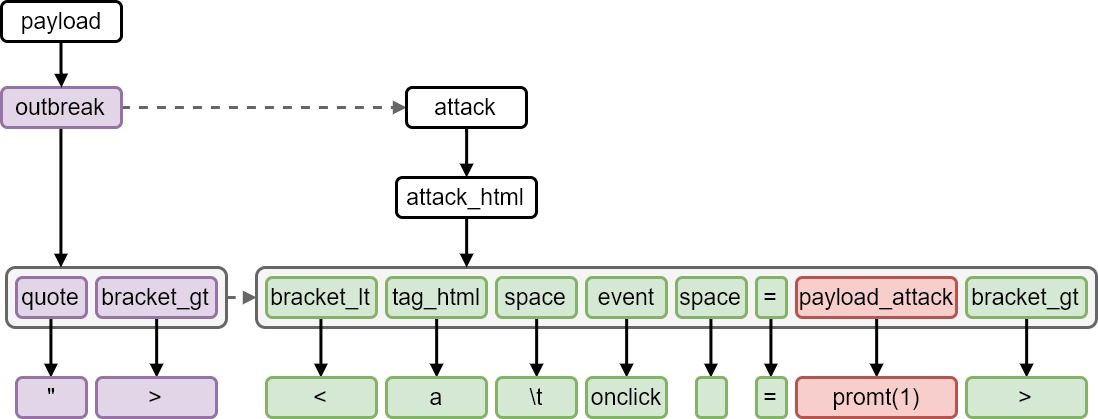
\includegraphics[width=\textwidth]{contents/images/DharmaPayloadConstructionExample.jpg}
	\caption{Dharma: Aufbau eines generierten Payloads}
	\label{fig:dharmaPayloadConstructionExample}
\end{figure}

\FloatBarrier
Diese werden in eine neue Regel ``+src\_value+'' übernommen\footnote{Die komplette Grammatikdefinition ist auf der GitHub-Projektseite von Dharma verfügbar \cite{Borgardt2017}.}.

Zum Schluss werden alle Sonder- sowie Leerzeichen durch die entsprechenden Regeln ersetzt. Die Generierung eines Payloads kann zur Verdeutlichung als Baumstruktur dargestellt werden. Abbildung \ref{fig:dharmaPayloadConstructionExample} veranschaulicht den abgearbeiteten Baumpfad von Dharma. Grau gestrichelten Pfeile symbolisieren aufeinanderfolgende Regeln, die nacheinander abgearbeitet werden. Volle Pfeile beschreiben eine direkte bzw. zufällige Auswahl von Dharma.

\subsubsection{Fuzzing/Mutation einzelner Elemente}

Da es in der Dharma-Implementierung nicht vorgesehen ist, eigene Methoden während der Generierung auszuführen, müssen alle Alternativdarstellungen für Zeichen in den Regeldefinitionen aufgeführt werden.

Ein Beispiel für verschiedene Zeichenkodierungen ist in Quelltext \ref{lst:xss.dg-<} aufgeführt. Einige Varianten der Zeichen können mit vorangestellten Nullen ausgedehnt werden. Daher ist die dazugehörige Regel ``zero'' ebenfalls aufgeführt.

\begin{lstlisting}[caption={Dharma: Regeldefinition des Zeichens ``<''},label=lst:xss.dg-<]
...
bracket_lt :=
<
\x3c
\x3C
\u003c
\u003C
%26%23x3c
%26%23x+zero+3c
%26lt
%26LT
%26LT%3B
%26lt%3B
%3C
&#60
&#+zero+60
...
zero :=
0
0+zero+
00+zero+
...
\end{lstlisting}


\subsubsection{Aufruf von Dharma}

Mit dem Befehl \textbf{\lstinline[language=bash]!python dharma.py -grammars grammars/xss.dg -count 1!} wird ein Payload vom Dharma-Generator unter Verwendung der oben beschriebenen Grammatikdefinition generiert. 

\begin{lstlisting}[caption={Dharma: Beispiel für einen generierten Payload},label=lst:DharmaXssOutput] 
\x3cimg+`\``&#0000062\u003cstyle+spacetype="text/css\'%26LTbody
{background:url("javascript:promt(\"dharmam')\')}\u003C/style>
\end{lstlisting}


Durch die kontextfreie Generierung werden in den meisten Fällen die Elemente, wie zum Beispiel Anführungszeichen, nicht paarweise gesetzt. Im Fall der generierten Payloads aus Quelltextbeispiel \ref{lst:DharmaXssOutput} wurde jeder Payload mit mehreren verschiedenen Anführungszeichen versehen. Dies hat zur Folge, dass der Browser den Quelltext nicht richtig interpretieren und somit den Quellcode nicht ausführen kann.

Mit der Abänderung von Konstruktionsregeln kann eine paarweise Generierung von Elementen erreicht werden. Im Quelltextbeispiel \ref{lst:dharmaPairwiseWorkaround} ist exemplarisch dargestellt, wie die Definitionsregeln aufgebaut werden müssen, um eine paarweise Generierung sicherzustellen. Ein solches Vorgehen würde die Grammatikdefinition aufblähen, da für jedes paarweise Zeichen eine neue Regel gepflegt werden müsste. Im Zuge dieser Arbeit wurde diese Eigenschaft des Dharma-Generators beibehalten, da hierdurch kontextfreie Payloads erstellt werden. 

\begin{lstlisting}[caption={Dharma: Beispiel einer paarweisen XSS-Grammatikdefinition},label=lst:dharmaPairwiseWorkaround]
%section% := value

payload :=
+attack+

attack :=
<div>+inner+</div>
<section>+inner+</section>

inner := ...

%section% := variance
main :=
+payload+
\end{lstlisting}

\paragraph{Hinweis:} Die verwendete Grammatikdefinition in dieser Arbeit nimmt fehlerhaften JavaScript-Code bei der Generierung mit Dharma in Kauf, weil die Transformation der aktuellen Grammatikdefinition in ein paarweise generierendes Äquivalent den zeitlichen Rahmen dieser Arbeit sprengen würde.

%%%%%%%%%% Smarty
\subsection{SmartGrazer: Kontextbasierter Generator ``Smarty''}\label{Smarty}

Der kontextbasierte Generator von SmartGrazer wird im folgenden als ``Smarty'' bezeichnet. Anders als bei Dharma werden für Smarty vordefinierte Payload-Grammatiken bereitgestellt. Diese enthalten keine Schleifen, sodass keine Mehrfachausführung einer Outbreak-Sequenz möglich ist. Smarty wählt aus einem Pool vordefinierter Payload-Muster ein zufälliges aus und befüllt dieses mit Elementen. Die definierten Payloads entsprechen hierbei im Grunde der selben Menge wie aus dem Kapitel \ref{Dharma}.

Als Vergleich zur beispielhaften Abbildung \ref{fig:dharmaPayloadConstructionExample} ist die selbe Payload-Definition im Smarty-Format in Abbildung \ref{fig:smartyPayloadConstructionExample} abgebildet.

\begin{figure}[htbp] 
	\centering
	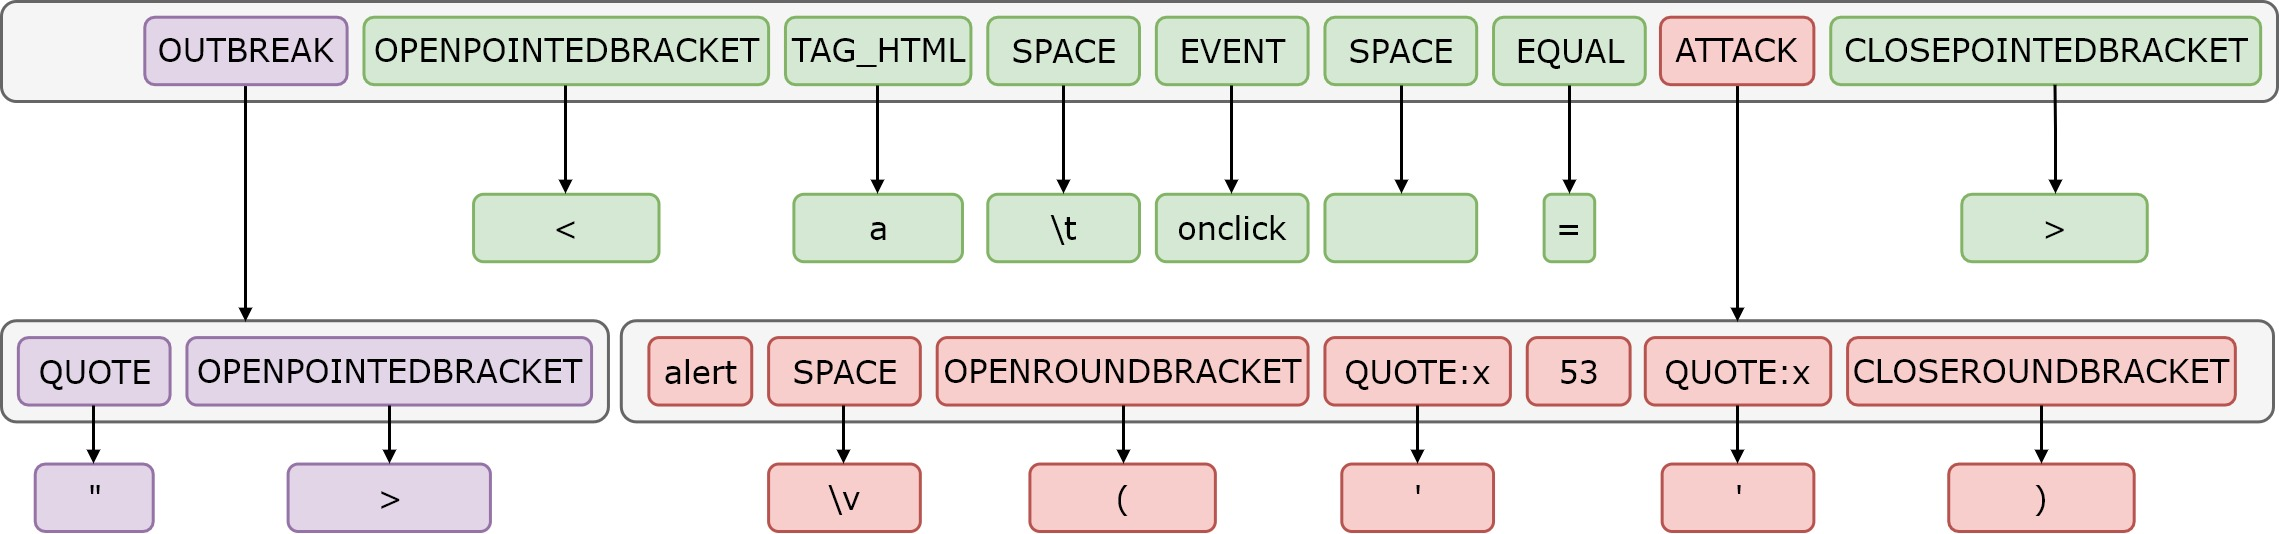
\includegraphics[width=\textwidth]{contents/images/SmartGrazerPayloadConstructionExample}
	\caption{Smarty: Aufbau eines generierten Payloads}
	\label{fig:smartyPayloadConstructionExample}
\end{figure}

\FloatBarrier
Smarty wurde mit einem Zwischenspeicher implementiert, sodass dem Generator mitgeteilt werden kann, welche Elemente zwar zufällig gewählt, aber paarweise zugewiesen werden sollen. In dem gezeigten Beispiel wurde definiert, dass die Anführungszeichen der ``ATTACK''-Sequenz immer gleich belegt werden sollen. Hierzu wird an das Schlüsselwort ``QUOTE'' eine generische Variable (hier: ``x'') mit einem vorangestellten Doppelpunkt angehängt. Das gewählte Zeichen für ``QUOTE'' in der OUTBREAK-Sequenz ist ohne Variable angeführt und kann somit jedes beliebige Element als Anführungszeichen enthalten.

\subsubsection{Payload Generierung}

Ein Payload wird zunächst als Angriffsmuster in der Konfigurationsdatei ``config/smarty/grammars.json'' definiert. Ähnlich wie bei der Dharma-Notation werden hier Elemente ebenfalls zu Gruppen zusammengefasst. In Abbildung \ref{lst:grammar-example} ist ein Angriffsmuster beispielhaft dargestellt. 

\begin{lstlisting}[caption={SmartGrazer: Auszug aus der Grammatik-Konfigurationsdatei},label=lst:grammar-example]
...
[
"OUTBREAK",
"OPENPOINTEDBRACKET",
"TAG_SCRIPT",
"CLOSEPOINTEDBRACKET",
"SPACE",
"ATTACK",
"OPENPOINTEDBRACKET",
"SLASH",
"TAG_SCRIPT",
"CLOSEPOINTEDBRACKET"
], ...
\end{lstlisting}

Schlüsselwörter, wie zum Beispiel ``OUTBREAK'' oder ``ATTACK'', werden während der Generierung in Objekte umgerechnet und deren Elemente in die Grammatik übernommen. Die dazugehörigen Definitionen befinden sich in den Dateien ``config/smarty/outbreaks.json'' und ``config/smarty/attacks.json''. Zum jetzigen Stand steht ein Schlüsselwort für eine Elementrepräsentation. Ein wiederholtes Anfügen von Outbreak-Objekten, wie bei Dharma, wurde nicht implementiert.

\subsubsection{Zeichen-Mutation}\label{ssec:payload-generation-mutation}

Ein Element innerhalb eines Payload wird bei dessen Ziehung mutiert, wenn dies für das Element in der Konfiguration erlaubt wurde. Diese Mutation gilt einmalig für den Payload und wird nach der Analyse der Antwort wieder verworfen. Hierdurch wird sicher gestellt, dass die Anzahl an gespeicherten Elemente konstant bleibt und nicht durch jede Mutation ein neues Element hinzukommt. Im Falle des Elements ``javascript'' sind zwei Mutations-Klassen implementiert:

\begin{description}
	\item[Uppy] Diese Mutationsklasse ändert die Groß- bzw. Kleinschreibung von Buchstaben in Zeichenketten. Beispiel: ``JaVaSCriPt''
	\item[Spacey] Diese Mutationsklasse fügt an einer zufälligen Stelle der Zeichenkette ein Leerzeichen ein. Beispiel: ``javas cript''
\end{description}
